 
In this Section we  give a brief and informal  overview of %the most salient features of  
\Chainmail -- a full exposition appears in Section \ref{sect:assertions}.
As well as   ``classical'' assertions \sophia{would be nice iof we had a better name}
 about  variables and the heap (\eg  \prg{a1}.\prg{myBank} = \prg{a2}.\prg{myBank}),
\Chainmail\ incorporates assertions   about
%
\textit{access},
% --- objects being accessible from other objects (\eg
% $\CanAccess{\x}{\y}$);
%
\textit{control} ,
% --- the next method to be invoked ($\Calls {\x} {\y} {\m} {\z}$);
%
\textit{authority},
%  --- about the change of some property (\eg $\Changes{\x.\f}$);
%
\textit{space} , %--- some property being observable within a subset of
%the current state ( $\Using{\A}{S}$);
%
and
%
\textit{time}.
% --- about some property holding in the future or in the past (\eg $\Future \A$ or $\Past \A$).
%



\sdparagraph{Configurations} We  will explain these concepts in terms of examples coming from  \prg{Bank}/\prg{Account} as  in the previous Section.
We will use the runtime configurations $\sigma_1$ and $\sigma_2$ 
shown in the left and right diagrams in Figure \ref{fig:BakAccountDiagrams}.
%These configurations could arise from the execution of different implementation of the \prg{Bank}/\prg{Account}
% module.
In both diagrams the rounded boxes depict objects:  green for those from the 
\prg{Bank}/\prg{Account}  module, and grey for the ``external'',  ``client'' objects.
The transparent green rectangle  shows which objects \prg{Bank}/\prg{Account}  module.
The object at \prg{1} is a \prg{Bank}, those at \prg{2}, \prg{3} and \prg{4} are 
\prg{Account}s, and those at \prg{91}, \prg{92}, \prg{93} and \prg{94} are 
``client'' objects which belong to classes different than those from the \prg{Bank}/\prg{Account}  module.

The configurations differ in the internal representation of the objects. 
Configuration  $\sigma_1$ may arise from execution using a module $M_{BA1}$, where  \prg{Account} objects of
  have a field \prg{myBank} pointing to their \prg{Bank}, and an integer field  \prg{balance}
-- the code can be found in xxx.\sophia{TODO add -- code is available somewhere}. 
Configuration  $\sigma_2$ may arise from execution using a module $M_{BA2}$,  where \prg{Account}s have a \prg{myBank}
field,  \prg{Bank} objects  have a \prg{ledger} implemented though a sequence of \prg{Node}s, each of which has a 
 field pointing to the \prg{Account}, a field \prg{balance}, and a field \prg{next}  -- the code can be found in yy.\sophia{TDOD add -- code is available somewhere}.

%In our diagrams. 
 
\begin{figure}[htbp]
\begin{tabular}{cc}
 \begin{minipage}{0.45\textwidth}
$\sigma_1$\\
 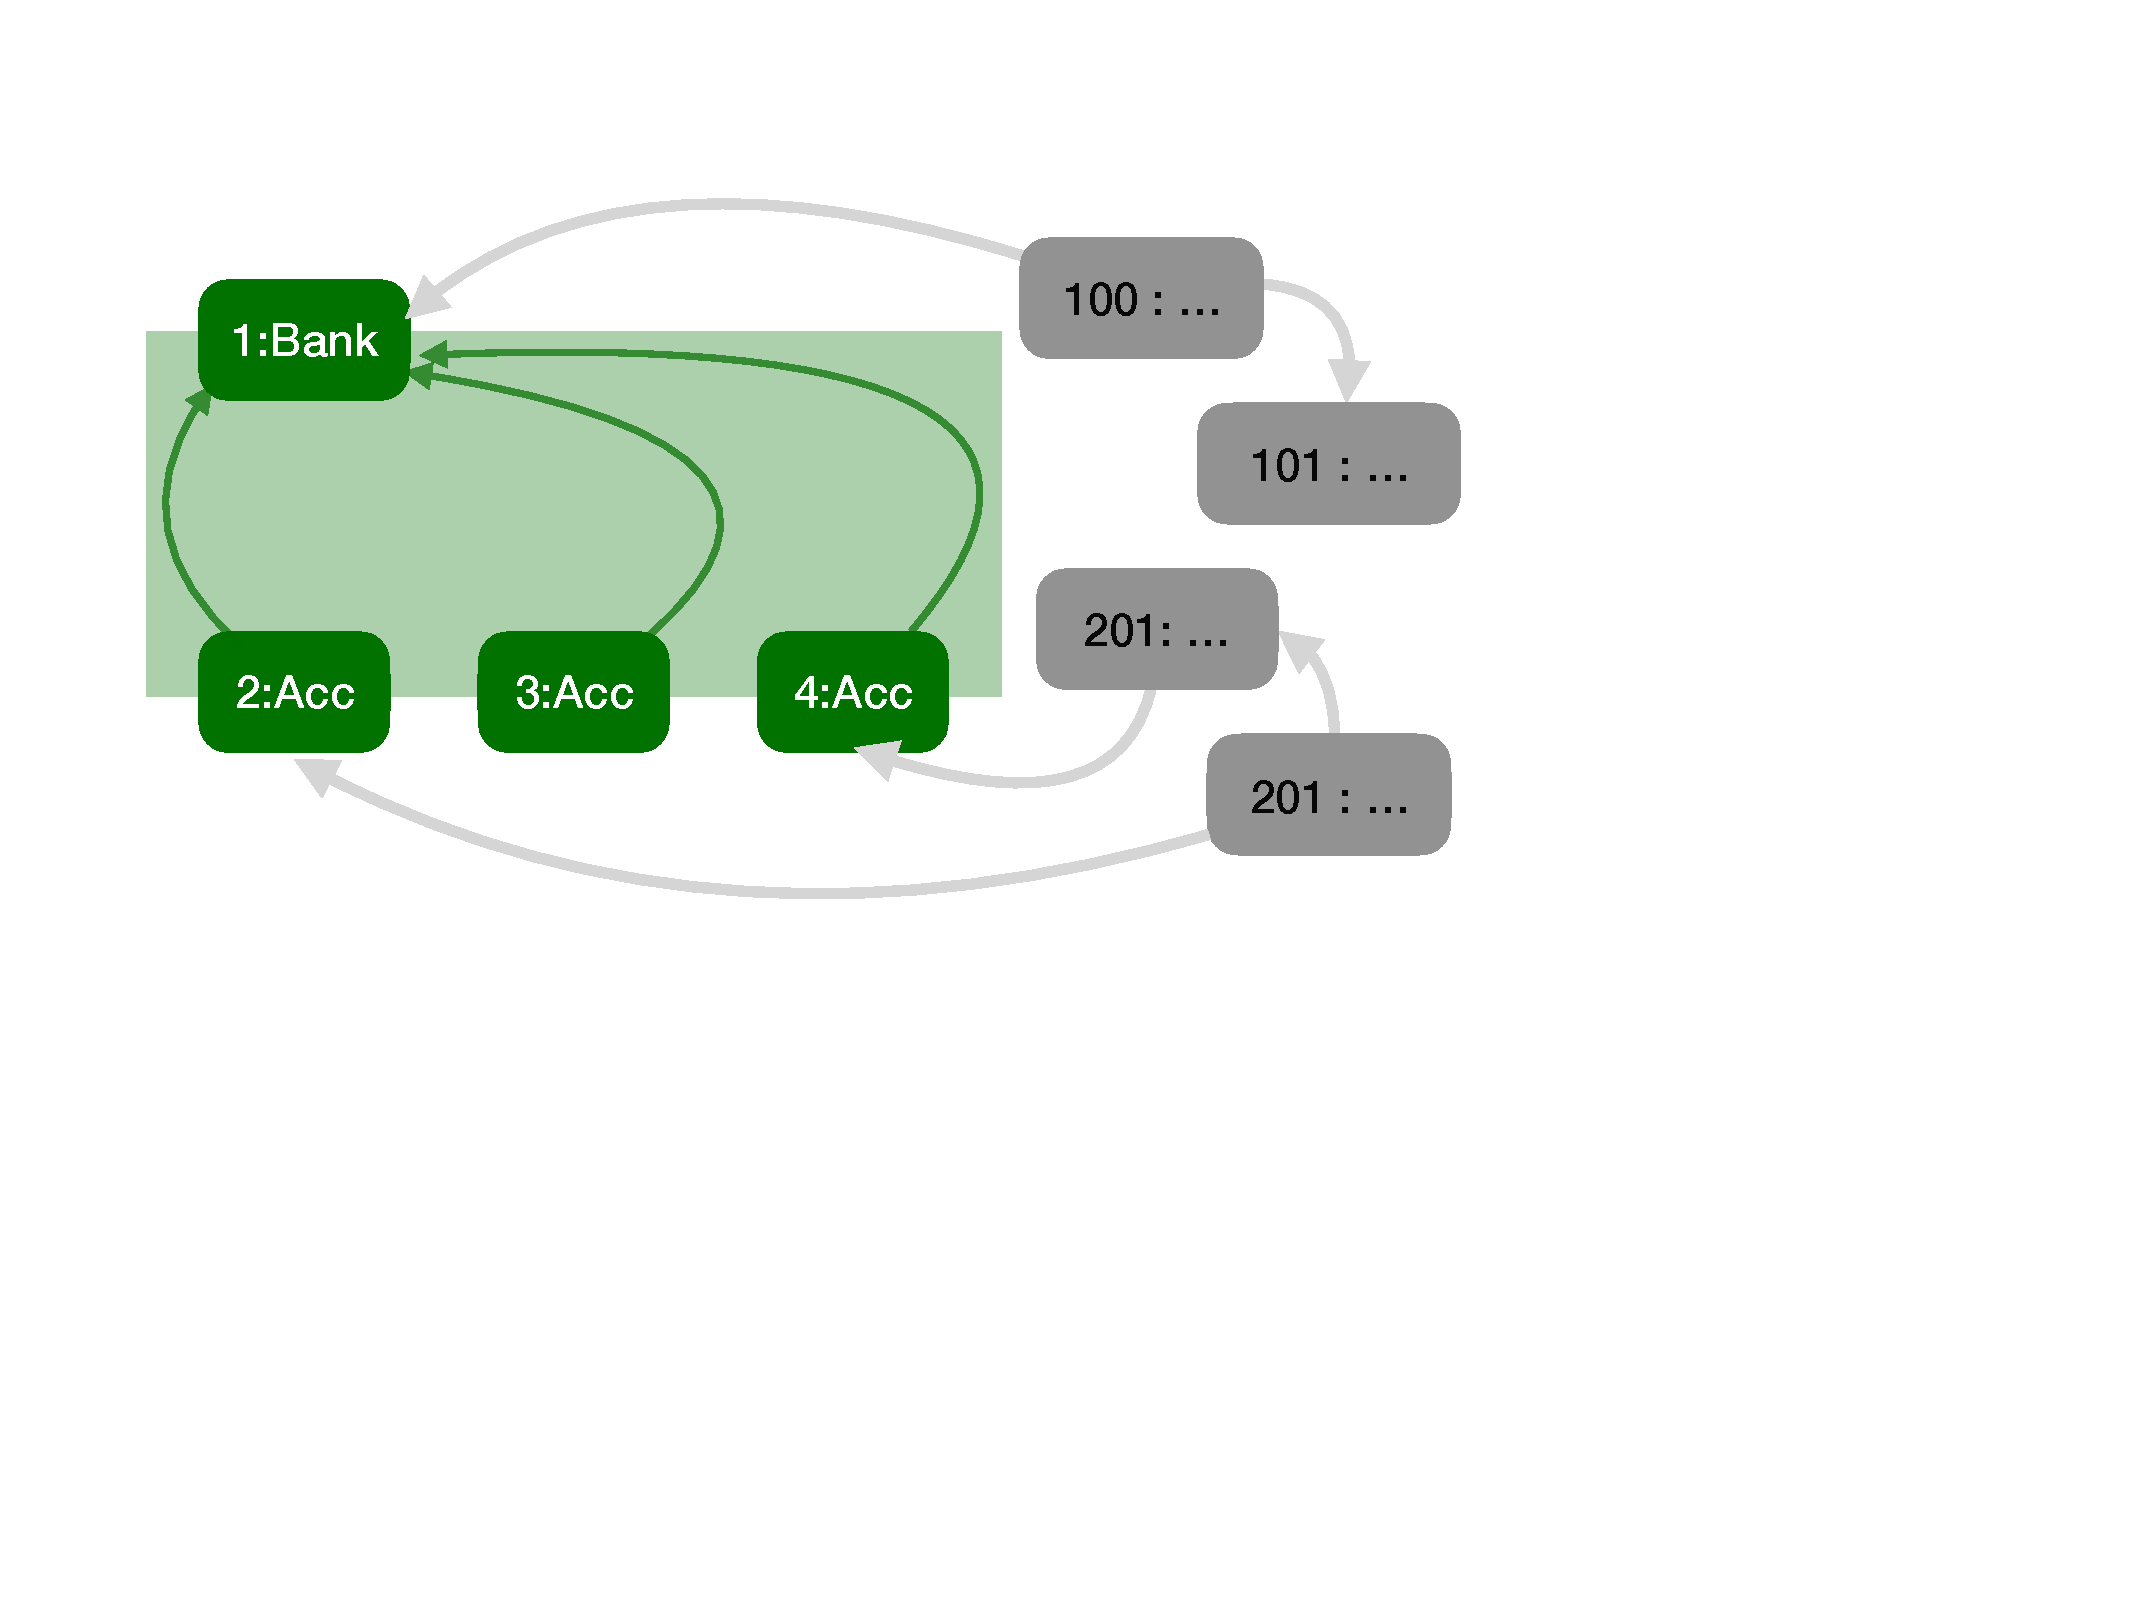
\includegraphics[width=\linewidth, trim=55  330 320 60,clip]{diagrams/BankAccount_version_1.pdf}
   \end{minipage}
 &  
 \begin{minipage}{0.45\textwidth}
 $\sigma_2$\\
  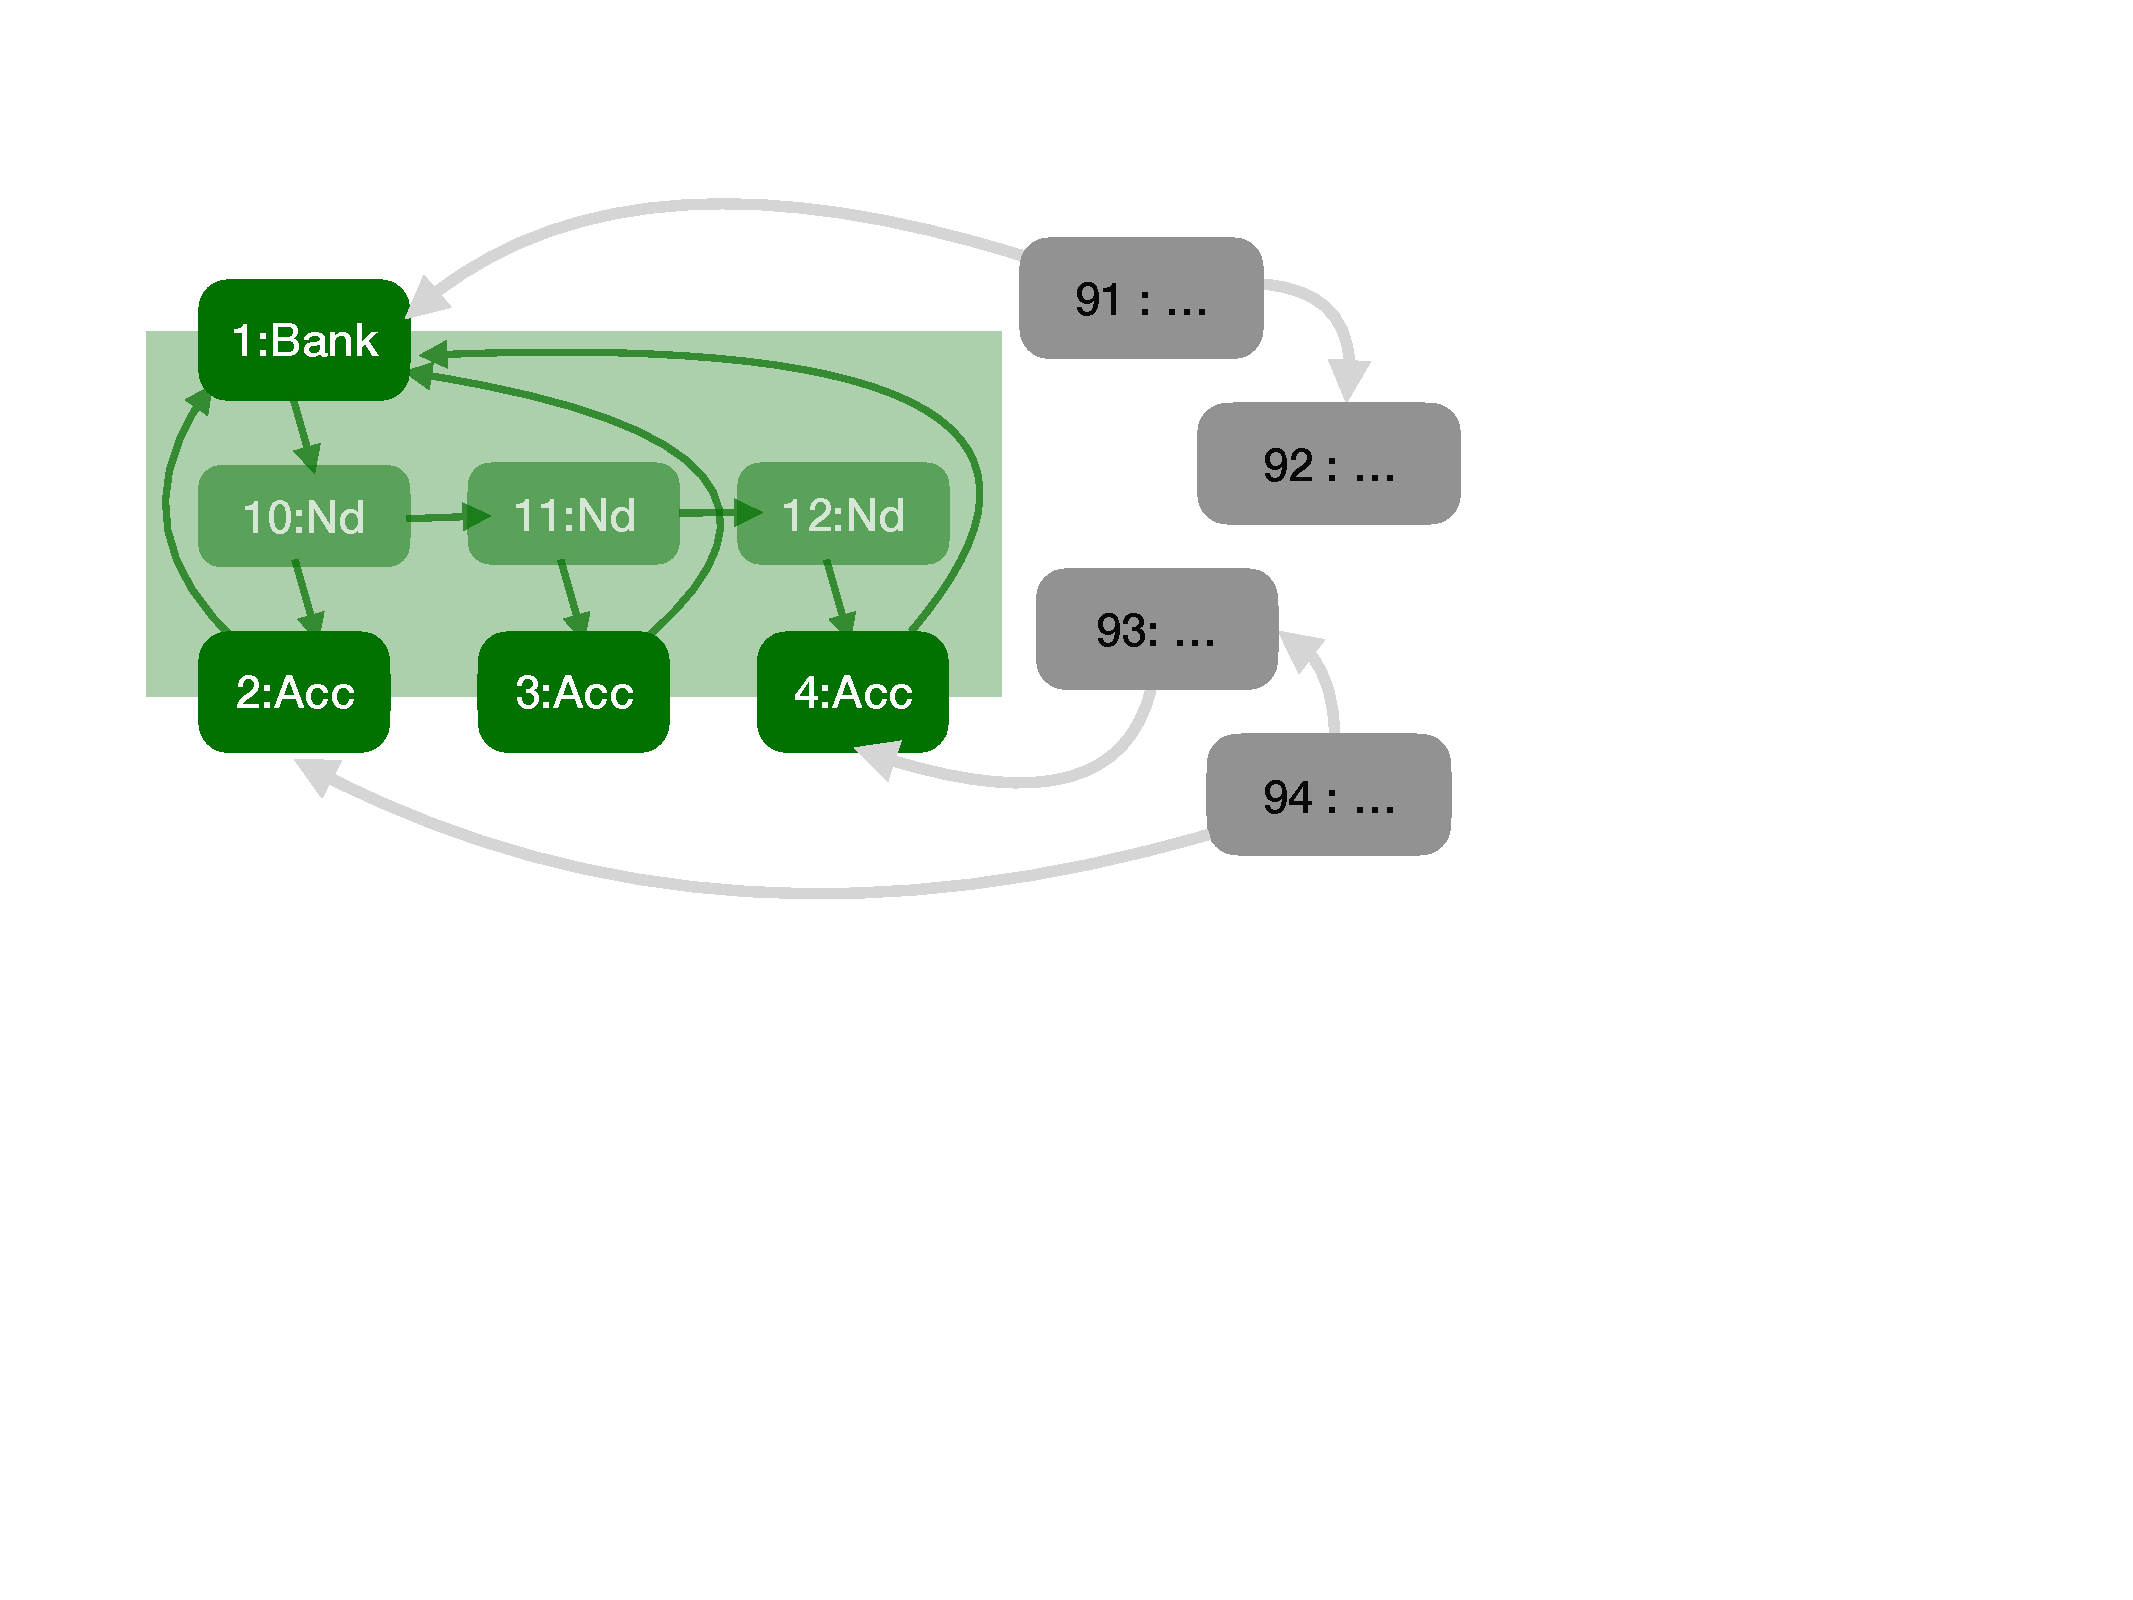
\includegraphics[width=\linewidth, trim=55  330 320 60,clip]{diagrams/BankAccount_version_2.pdf}
   \end{minipage}
\end{tabular}
\caption{Two runtime configurations for the \prg{Bank}/\prg{Account} example. 
}
\label{fig:BakAccountDiagrams}
\end{figure}

\noindent 
For the rest,  assume variable identifiers $\prg{b}_1$, and $\prg{a}_2$--$\prg{a}_4$, and  $\prg{u}_{91}$--$\prg{u}_{94}$ denoting objects \prg{1}, \ \prg{2}--\prg{4},
and   \prg{91}--\prg{94} respectively for both $\sigma_1$ and $\sigma_2$.
That  is, $\sigma_i(\prg{b}_1)$=\prg{1}, and 
$\sigma_i(\prg{a}_2)$=\prg{2}, $\sigma_i(\prg{a}_3)$=\prg{3},  $\sigma_i(\prg{a}_4)$=\prg{4}, and  
  $\sigma_i(\prg{u}_{91})$=\prg{91}, $\sigma_i(\prg{u}_{92})$=\prg{92},   
  $\sigma_i(\prg{u}_{93})$=\prg{90}, $\sigma_i(\prg{u}_{94})$=\prg{94},
  for $i$=$1$ or $i$=$2$.


% X Y Z W
% Z: top
% LEFT
  
%%Unlike JML or Dafny \cite{Leavens-etal07,dafny} \Chainmail specifications are not
%%tied tightly to the systems they are specifying.
%%\sdcomment
%%\sophia{Not sure what this means.}
%% Rather, a system may
%%be described by a set of \Chainmail\ specifications, each consisting of
%%a number of named \lstinline+policy+ clauses.
%%%\sdcomment
%%\sophia{We do not have that 
%%syntax any more. Do we need it?}
%\Chainmail\ specifications and policies overlap and are interlinked to
%provide strong protection against attacks --- just like the links in
%physical chainmail.
%%\sdcomment
%\sophia{What does overlap mean?}
%Each policy should aim to capture one very
%specific concern in the design of a system. 
%%\sdcomment
\sophia{I think this para is great -- not sure it belongs here. \\
While traditional policies are
expressed as Hoare triples --- often describing a single method
invocation on an instance of the class being specified (as in
XXXXX), R%Figure~\ref{BANK-OR-DOM}).  
holistic policies are expressed as 
temporal or spatial invariants that a module that
conforms to the specification must maintain even though any other code
may be executed (as in the three policies in section~\ref{DOM-OR-BANK}).}

%% \Chainmail\ policies (and specifications) can cross cut both each
%% other and the various modules and objects in the system being
%% specified.  The validity of a specification is the conjunction of its
%% policies; a module or an object must satisfy all the specification's
%% policies for us to consider that the object meets the specification.
%% Policies and specifications are not tied to any specific module or
%% class: rather, any implementing module that satisfies the
%% specification's policies obeys the specification.

% \sd{\Chainmail~specifications ere we need a summary of what will come.}
%\Chainmail can express necessary specifications because its invariant
%language includes \kjx{several carefully-chosen} \textit{holistic}
%assertion constructs, along with traditional state-based assertions.
%%\jncomment
%\james{if we say things like that, need to discuss alternative
%  constructs in the discussion section. do we have alternatives?
%  transitive Access. two-state assertions. what else? \sd{that would be good, but 
%  more work to do. Can some body do it? Is it very important to have?}}.
%That is, as well as supporting assertions on the contents of local
%variables and object fields (\eg $\prg{x}.\f1 > \prg{this}.\f2$),
%\Chainmail\ incorporates assertions which talk about
%%
%\textit{access}
%--- objects being accessible from other objects (\eg
%$\CanAccess{\x}{\y}$);
%%
%\textit{control} --- the
%next method to be invoked ($\Calls {\x} {\y} {\m} {\z}$);
%%
%\textit{authority} --- about the change of some
%property (\eg $\Changes{\x.\f}$);
%%
%\textit{space} --- some property being observable within a subset of
%the current state ( $\Using{\A}{S}$);
%%
%and
%%
%\textit{time} --- about some property
%holding in the future or in the past (\eg $\Future \A$ or $\Past \A$).
%%
%.
%%\scd
%  \sophia{While
%many  individual
%features of \Chainmail can  be found also in other work, we
%%claim that their  combination as well as
%%their application in the specification of open systems are novel.
%argue that their power and novelty for specifying open systems lies in their careful
%  combination}
%  %\kjx
%  \james{Hmm. a delicate, subtle argument \ldots }
%%
%%
%These assertions draw from some concepts from object capabilities
%($\CanAccess{\_}{\_}$  for  permission and $\Changes{\_}$ for
%authority) 
%as well as temporal logic ($\Future \A$, $\Past \A$ and friends), and the relation of
%our spatial connective ($\Using{\A}{S}$)  with ownership and effect
%systems.
%%\sdcomment
%\sophia{TODO: add references here}. 
%%\jncomment
%\james{don't forget the whole
%  AOP mionitoring/specs stuff, just for fun.  (HELM contracts!!! (vs
%  Meyer Contracts :-)}  
%%
%%\jncomment
%\james{somewhere, should we say something like: the goal is
%  to allow wholistic specifations with as extra little machinery as
%  possible over a basic Hoare language}.
\sdparagraph{Classical Assertions} talk about the contents of the 
local variables (\ie the topmost stack frame), and the 
fields of the various objects (\ie the heap).  
  For example, the assertion that  $\ \prg{a}_2.\prg{myBank}$=$\prg{a}_3\prg{myBank} \ $, expresses that 
  $\prg{a}_1$ and  $\prg{a}_2$  have the same bank. In fact, this assertion is
  satisfied in both $\sigma_1$ and $\sigma_2$, written formally as\\
  $\strut$ \hspace{2cm}  $...,\sigma_1 \ \models \ \prg{a}_2.\prg{myBank}=\prg{a}_3.\prg{myBank}$\\
  % , $\ \ \ $  and also 
  $\strut$ \hspace{2cm}  $...,\sigma_2 \ \models \ \prg{a}_2.\prg{myBank}=\prg{a}_3.\prg{myBank}$
   
 
  The term \prg{x}:\prg{ClassId} says that \prg{x} is an object of class \prg{ClassId}. For example\\
  $\strut$ \hspace{2cm}  $...,\sigma_1 \ \models \ \prg{a}_2.\prg{myBank}=\prg{a}_3.\prg{myBank}$.
  
  We support ghost fields,\sophia{TODO citation}
    \eg $\prg{a}_1$.\prg{balance} is a ghost field in $\sigma_2$ since \prg{Account}s do not store 
  a \prg{balance} field. But its value can be defined so that for any \prg{a} of class \prg{Account} the value
  of \prg{a.balance} is
   \prg{nd}.\prg{balance} such that \prg{nd} is a \prg{Node}, 
   and \prg{nd}.\prg{myAccount}=\prg{a}.\sophia{All hell is loose here, as ghostfields require recursive defs, but I want to postpone these.}
%  $\prg{a}.\prg{balance}$=\prg{m} if
%  \prg{a.myBank.next}$^k$.\prg{acc}=\prg{a}, and  \prg{a.myBank.next}$^k$.\prg{balance}=


We also support the usual logical connectives, and so, we can express assertions such as \\
$\strut$ \hspace{2cm}    $\forall \prg{a}. [ \ \ \prg{a}:\prg{Account} \ \longrightarrow \ \ \prg{a}.\prg{myBank}:\prg{Bank}\ \wedge\  \prg{a}.\prg{balance}\geq 0\ \ ] $ .



\sdparagraph{Permission: Access}

Our first holistic assertion $\CanAccess{\x}{\y}$ asserts that one
object $\x$ has a direct reference to another object $\y$: either one
of $\x$'s fields contains a 
reference to $\y$, or the receiver of the currently executing method is \prg{x}, and \prg{y}
is one of the arguments or a local variable. 
For example:\\
 $\strut$ \hspace{2cm}  $...,\sigma_1 \ \models \  \CanAccess{\prg{a}_2}{\prg{b}_1}$

This assertion can be used to make assertions about heap structures (and thus
object values), for example if a \prg{cacheValid} field is true,
then that object can access to a cached value:

\begin{lstlisting}
  a.cacheValid == true `$\weakImplies \CanAccess(a)(cacheValue)$` 
\end{lstlisting}

%\kjx
\james{do we really not also need reachable (transitive closure of access)}
\susan{we don't seem to need transitivity in any of the examples}


\sdparagraph{Control: Calls}

The  $\Calls {\x} {\y} {\m} {\z}$
assertion is more-or-less the control flow analogue of
the access assertion, and is true 
in program states where a method on object 
${\x}$ makes a method call ${\y}.{\m}({\z})$ --- that is it calls method 
{\m} on object {\y} with arguments {\z}.


\begin{lstlisting}
   another illustrative example, presumably in the context of the
   running example from the intro. which we need to pick first.
\end{lstlisting}


\paragraph{Authority Changes}

The $\Changes{\x.\f}$  assertion is true when the value of \prg{x.f}
in the next state is different to the value in the current state.
For example, we 

\begin{lstlisting}
   another illustrative example, presumably in the context of the
   running example from the intro. which we need to pick first.
\end{lstlisting}

\paragraph{Space: With}

The space assertionn $\Using{\A}{S}$ states the some assertion $\A$ is
true when the heap used by that assertion is restrcited to the
footprint $\S$  
%\kjx
\james{footprint F?}.

%\kjx
\james{OK someone needs to explain what that's for and when/why it is sound to
do it}

\begin{lstlisting}
   another illustrative example, presumably in the context of the
   running example from the intro. which we need to pick first.
\end{lstlisting}


\paragraph{Time: Next, Will, Prev, Was}

\Chainmail supports several temporal operators familiar from temporal
logic ($\Future \A$ or $\Past \A$ or $\Next \A$ or $\Prev \$A$). 
We support birectional temporal
assertions, constraining either future ($\Future \A$. $\Next \A$)
or past behaviour ($\Past \A$.  $\Prev \$A$) either considering only
the  immediate next or immediate previous step ($\Next \A$,
$\Prev \$A$) or for conditions that become eventually true in some
distant future, or were true once in some distant past  
($\Future \A$, $\Past \A$). We have bidirectional pairs of operators
to give expressiveness in writing assertions: this does not offer any
additional reasoning power. 

For example, a part of the observer pattern is that when
a subject is notified of a change, then the observer must
be told to update itself.    We can write this from the
subject's perspective, looking forwards:

\begin{lstlisting}
  Call(_,subject,notify,_) --> Will(Call(subject,observer,update,_))
\end{lstlisting}

\noindent meaning that once notify is called on a subejct, then its
observer will be updated sometime in the future.  We can write a very
similar specification for an observer, looking backwards.

\begin{lstlisting}
  Call(subject,observer,update,_) --> Was(Call(_,subject,notify,_))
\end{lstlisting}

\noindent meaning that if a subject updates an observer, that subject
have been notified sometime previously. We could tighten each
specifaction, so that the update must immediately follow the
notification, by replacing $\Future \A$ or $\Past \A$ with 
$\Next \A$ or $\Prev \A$.

%\kjx
\james{bother. should probably do time earlier, because most of the
   example assertions I can think of a things like
   \lstinline+(change(x.f) ->  past(call(_,xm,_)+ which needs the temporal operator}

 
\sophia{While
many  individual
features of \Chainmail can  be found also in other work, we
%claim that their  combination as well as
%their application in the specification of open systems are novel.
argue that their power and novelty for specifying open systems lies in their careful
  combination}
  %\kjx
  \james{Hmm. a delicate, subtle argument \ldots }
%
%
These assertions draw from some concepts from object capabilities
($\CanAccess{\_}{\_}$  for  permission and $\Changes{\_}$ for
authority) 
as well as temporal logic ($\Future \A$, $\Past \A$ and friends), and the relation of
our spatial connective ($\Using{\A}{S}$)  with ownership and effect
systems.
%\sdcomment
\sophia{TODO: add references here}. 
%\jncomment
\james{don't forget the whole
  AOP mionitoring/specs stuff, just for fun.  (HELM contracts!!! (vs
  Meyer Contracts :-)}  
%
%\jncomment
\james{somewhere, should we say something like: the goal is
  to allow wholistic specifations with as extra little machinery as
  possible over a basic Hoare language}.

